                               %----------------------------------%
                               % Manhattan College Math Dept      %
                               % Student Homework Template v1     %
                               %    R. Goldstone, 1/1/2011        %
 	               % Edited by T. McGrail, 2/11/2011  %
 	               % Edited by R. McGovern, 8/16/2011 %
 	               % Edited by J. Kirtland, 1/20/2015 %
                               %----------------------------------%
% PREAMBLE ============================================================================

\documentclass[12pt]{article}
\usepackage[utf8]{inputenc}    % set input encoding so bullets are printed
\usepackage{amssymb,amsmath,amsthm}
\usepackage{listings}
\usepackage[usenames,dvipsnames]{color}
\usepackage{matlab-prettifier}
\usepackage{graphicx}

 
% FILL-IN, THEN GO TO DOCUMENT MAIN BODY **********************************************
% TEXWORKS: USE CTRL-TAB TO JUMP FROM INPUT FIELD TO INPUT FIELD
\newcommand{\myname}{Amy Pitts} % Enter name
\newcommand{\duedate}{February 30, 2019} % Enter date, e.g., April 1
\newcommand{\courseno}{440L}      % Enter course number (just the number)
\newcommand{\coursename}{Machine Learning}    % Enter course name
\newcommand{\instructorname}{Instructor: Dr. Pablo Rivas} % Enter instructor name
\newcommand{\assignumber}{2}   % Enter assignment number#.
\newcommand{\exerciselist}{Chapter 2,3}      % Enter problem references.  Give a complete list, in order, of all of the problems that you will do on this assignment.  Use the format 2.20 to designate problem  # 20 from chapter 2 of the text.
\newcommand{\spacingfactor}{2}
% END FILL-IN *************************************************************************

% DOCUMENT STRUCTURES -----------------------------------------------------------------

% PAGES
\usepackage[paper=letterpaper, margin=1in, headsep=20pt]{geometry}
  
\newcommand{\firstpageinfo}  
    {\textsf{\large\myname}    \hfill     Math \courseno{:}\,\coursename \\
  Assignment Number \assignumber \hfill  Due:  \duedate \\
  \instructorname}
% END PAGES

% HEADERS AND FOOTERS
\usepackage{fancyhdr}
\pagestyle{fancy}              % Headers and footers for page 2 and beyond
  \lhead{\textit{\myname}}
  \chead{\textit{Math \courseno}}
  \rhead{\textit{\textit{Assignment Number \assignumber}}}
  \cfoot{\textit{\thepage}}
  \renewcommand{\headrulewidth}{0.4pt}
% END HEADERS AND FOOTERS

% TEXT SPACING
\usepackage{setspace}   %Allows for Doublespacing
\usepackage{ifthen}   %Used to create a response environment
% END TEXT SPACING

% PROBLEM AND RESPONSE ENVIRONMENTS
 \newcommand\myqed{}                 % creates command for tombstone at end of proof
\newcommand{\printmyqed}[1][]       % decides whether to print tombstone or not
  {%
  \ifthenelse{\equal{#1}{Proof}}
  {\renewcommand{\myqed}{\qed}}
  {\renewcommand{\myqed}{}}
  }

\newenvironment{exercise}[1][]{%
  \bigskip                          % Space before problem statement
  \noindent \textsf{Exercise #1.}\slshape }{}
   
\newenvironment{response}[1][\textit{Solution}]{%
  \printmyqed[#1]
  \begin{spacing}{\spacingfactor}
  \medskip                          % Space before solution
  \noindent \textit{#1.}}{\myqed\end{spacing}\medskip\hrule}
% END PROBLEM AND RESPONSE ENVIRONMENTS

% =====================================================================================

\begin{document}
\thispagestyle{empty}

% TOP MATTER --------------------------------------------------------------------------
\noindent\firstpageinfo
\begin{center} \underline{\textsf{Exercise List}}\\[5pt] \exerciselist \end{center}
\medskip\hrule
% END TOP MATTER ----------------------------------------------------------------------


%----------------------------------------------------------------------------------------
\begin{exercise}[1] % Put problem reference inside the brackets
  Use sklearn's implementation of k-Nearest Neighbors for 
  regression purposes,  which is found in sklearn.neighbors.KNeighborsRegressor.
  You will find the best value of k using 10 fold CrossValidation 
  (CV), which is found in sklearn.model\_selection.KFold.
  \begin{enumerate}
    \item[a)]  You will modify the python code below to generate 1000 data points, or alternatively you could
    use part of your semester project dataset if it is related to regression.
  \lstset{language=Python,frame=single}
  \begin{lstlisting}[language=Python,frame=single]
import numpy as np
from matplotlib import pyplot as plt

def genDataSet (N) :
    x = np . random . normal (0 , 1 , N)
    ytrue = (np.cos ( x ) + 2) / (np.cos ( x * . 4 ) + 2)
    noise = np . random . normal (0 , 0 . 2 , N)
    y = ytrue + noise
    return x , y , ytrue

x , y , ytrue = genDataSet(100)
plt.plot(x , y , '.')
plt.plot(x , ytrue , 'rx')
plt.show( )
  \end{lstlisting}
  \item[b)]Using 10-fold CV, you will report the three best values of k-neighbors that yield the best CV
  E$_{out}$. You will vary the values of k in the following range: $k = 1 ,3,5,\dots 2[\frac{N+1}{2}]-1$.
  \item[c)] You will report the best CV E$_{out}$. 
  \end{enumerate}
\end{exercise}
  
  
\begin{response}[Solution]
  \textbf{a)} 
  \lstset{language=Python,frame=single}
  \begin{lstlisting}[language=Python,frame=single]
import numpy as np
from matplotlib import pyplot as plt

def genDataSet (N) :
    x = np . random . normal (0 , 1 , N)
    ytrue = (np.cos ( x ) + 2) / (np.cos ( x * . 4 ) + 2)
    noise = np . random . normal (0 , 0 . 2 , N)
    y = ytrue + noise
    return x , y , ytrue

x , y , ytrue = genDataSet(1000) #changed this number to 1000
plt.plot(x , y , '.')
plt.plot(x , ytrue , 'rx')
plt.show( )
  \end{lstlisting}
  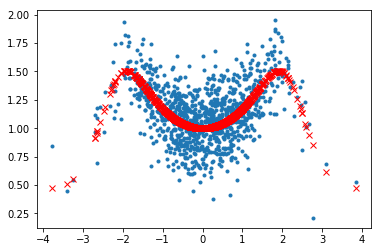
\includegraphics[width=100mm]{1a.png}

  \textbf{b) and c)} 
  \lstset{language=Python,frame=single}
  \begin{lstlisting}[language=Python,frame=single]
from sklearn.neighbors import KNeighborsRegressor
from sklearn.metrics import mean_squared_error
from sklearn.model_selection import KFold
kf = KFold(n_splits=10)
X = np.array([x,y]).T
kf.get_n_splits(X)
  
msek = {}
bestk= 0
bestmse = 100000
for k in np.arange(1,2*np.floor(((len(ytrue)*0.9)+1)/2)-1,2):
  print(k)
  mse = []
  for train_index, test_index in kf.split(X):
    X_train, X_test =     X[train_index],     X[test_index]
    y_train, y_test = ytrue[train_index], ytrue[test_index]
    neigh = KNeighborsRegressor(n_neighbors = int(k))
    neigh.fit(X_train, y_train) 
    predict = neigh.predict(X_test) 
    mse.append(mean_squared_error(y_test, predict))
  print(np.mean(mse))
  msek[k] = np.mean(mse)
  #part c
  if bestmse > msek[k]:
      bestmse = msek[k]
      bestk = k
      print(k)
      print(bestmse)
  plt.plot(k,msek[k],'r.') #mse

plt.show()
print(bestk)
  \end{lstlisting}

  The best three best $k$ using mse as an evaluation metric are:
  \medskip

    \begin{tabular}{ |c |c |c|c| } \hline
      $k$ & 1.0 & 3.0 & 5.0 \\ \hline
      MSE & 0.00045241177636707794 & 0.000512687006146458 & 0.0006638327509173002\\  \hline
    \end{tabular}
   \medskip

   This can also be seen by plotting the MSE by $k$. \\
   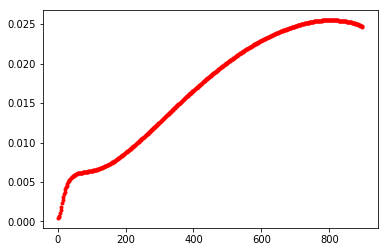
\includegraphics[width=100mm]{1b.png}

   The smallest MSE is the best, making smaller $k$s better then
   larger $k$s. 
\end{response}
%------------------------------------------------------


\begin{exercise}[2] % Put problem reference inside the brackets
  Using the same dataset you just tried in the previous problem, repeat the experiment
  100 times storing the best three $k$ number of neighbors in every single trial, and at the end of all trials
  plot a histogram of all the values of $k$ that you saved.
\end{exercise}
   
\begin{response}[Solution] 
  \lstset{language=Python,frame=single}
  \begin{lstlisting}[language=Python,frame=single]
from sklearn.neighbors import KNeighborsRegressor
from sklearn.metrics import mean_squared_error
from sklearn.model_selection import KFold

kf = KFold(n_splits=10)
bestkall = []
for i in range(100):
  x, y, ytrue = genDataSet(1000)
  X = np.array([x,y]).T
  kf.get_n_splits(X)
  
  msek = {}
  bestk= 0
  bestmse = 100000
  for k in np.arange(1,2*np.floor(((len(ytrue)*0.9)+1)/2)-1,2):
    mse = []
    for train_index, test_index in kf.split(X):
      X_train, X_test =     X[train_index],     X[test_index]
      y_train, y_test = ytrue[train_index], ytrue[test_index]
      
      neigh = KNeighborsRegressor(n_neighbors = int(k))
      neigh.fit(X_train, y_train) 
      predict = neigh.predict(X_test) 
      mse.append(mean_squared_error(y_test, predict))
    msek[k] = np.mean(mse)
    if bestmse > msek[k]:
      bestmse = msek[k]
      bestk = k
      print(k)
      print(bestmse)
    bestkall.append(bestk)
plt.hist(bestkall)
  \end{lstlisting}
  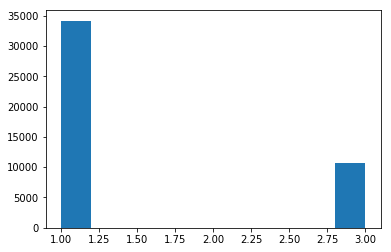
\includegraphics[width=100mm]{2.png} 
\end{response}


%------------------------------------------------------

\begin{exercise}[3] % Put problem reference inside the brackets
  \textbf{Experiment with k-means for color quantization.} \\
  Using sklearn’s implementation of k-means, find the best color 
  clustering for an image of your choice. A good portrait of yourself 
  could be fun (just sayin’). Color quantization is the science behind 
  compression of images. The idea is to represent an image with 
  fewer colors than the original. The experiment consists of the 
  following steps:
  \begin{enumerate}
    \item[a)] Download to your computer the file hw3.kmeans.img.py
    \item[b)] In the same folder where you downloaded the program, 
    save a copy of your picture for experimentation.\item[c)] Go to line 23 and set n\_colors with your choice of a number of colors between 2 and 64. This
    number is actually the number of clusters (or k) we are searching for in an unsupervised manner
    using kmeans.
    \item[d)]  Then go to line 25 and replace the image file name with the name of your image file. This is
    where your image is read into a numpy array.
    \item[e)] Run the program. Observe the result. If the result does not look funny to you, repeat from 3.(c)
    until it does. Then, report your result image along with your answers to the following questions:
    \begin{enumerate}
      \item[i)] Explain what happens when you increase or decrease the value of n\_colors?
      \item[ii)] Explain in what other possible applications do you think this can be useful?
      \item[iii)] Why do you think the resulting picture was funny at the end?
    \end{enumerate}
  \end{enumerate}
\end{exercise}
   
\begin{response}[Solution] This is my puppy Penny \\
  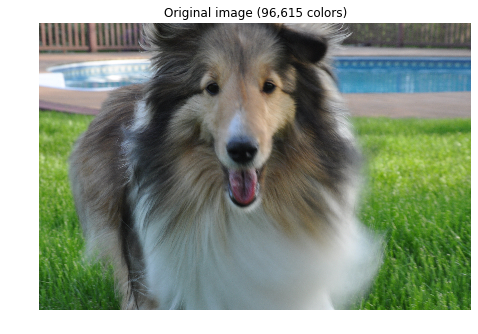
\includegraphics[width=85mm]{3_1.png} 
  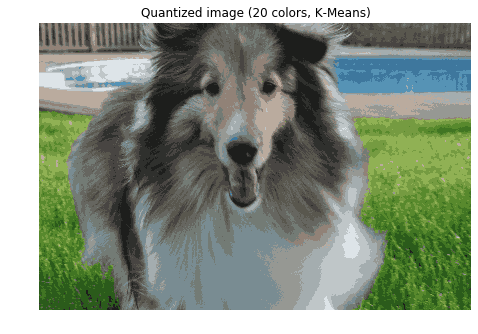
\includegraphics[width=85mm]{3_4.png} 
  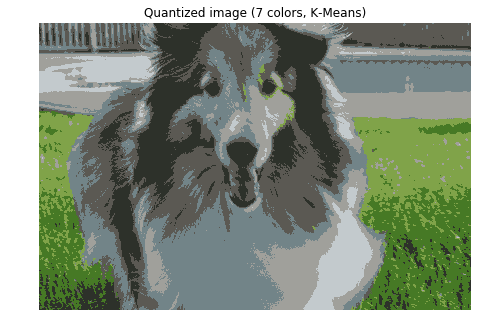
\includegraphics[width=85mm]{3_2.png}
  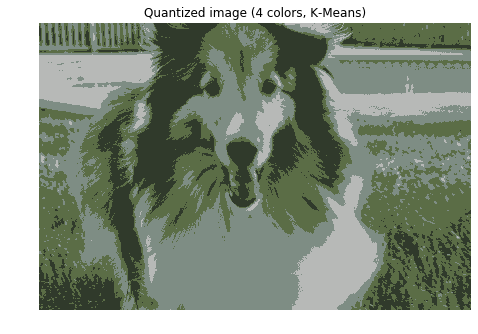
\includegraphics[width=85mm]{3_3.png}

  \textbf{i)} When I increase the n\_color there are more 
  colors in the picture, when I decrease it there are less 
  colors. When there is only 2 n\_colors then the picture 
  has only two colors which end up being the averages of 
  two groups of colors related to eachother 

  \textbf{ii)} This would be helpful in displaying images 
  on devices that do not have the ability to represent a lot 
  of different colors. It decreases the complexity and it only 
  takes away some of the detail. One place were this is helpful 
  is on old video game hand held devices. 

  \textbf{iii)} The picture looks cool to me. It is more cartoon-ish 
  but less bright with color. With less group the color turns 
  more grayish green and more washed out. 
  
  
\end{response}

%------------------------------------------------------


\begin{exercise}[4] % Put problem reference inside the brackets
  \textbf{Neural networks: The MLP}
  \begin{enumerate}
    \item[a)] Download the python program hw3.MLP.sol.py which implements a 
    10 fold cross validation approach to find the best number of 
    neurons and the best learning parameter $\eta$ (eta) in an MLP
    for regression. For learning purposes you could download hw3.MLP.py first, which is a simple
    implementation of the MLP.
    \item[b)] Download the python program hw3\_4\_a\_gendata.py which generates random data.
    \item[c)] Run the program in 4.(a) for 1,000 samples, and then take note of the best number of neurons
    and $\eta$. Go here https://goo.gl/forms/QFmaNWYaFLcPWdim2 and report your results. You can
    do it as many times as you want, but at least one is required. 
    \item[d)] Explain your results. What do you think is happening? What is your interpretation of the
    number of neurons with respect to the performance of the network?
    \item[e)]  (extra credit) Repeat 4.(c)-(d) but for 10,000 samples.
  \end{enumerate}
\end{exercise}
   
\begin{response}[Solution] 
  \textbf{a)}
  \lstset{language=Python,frame=single}
  \begin{lstlisting}[language=Python,frame=single]
import hw3_4_a_gendata
import numpy as np
import matplotlib.pyplot as plt
from sklearn.neural_network import MLPRegressor
from sklearn.model_selection import KFold
# generates data & split it into X (training input) and y (target output)
X, y = hw3_4_a_gendata.genDataSet(100)
neurons = 1000  # <- number of neurons in the hidden layer
eta = 0.01       # <- the learning rate parameter
# here we create the MLP regressor
mlp =  MLPRegressor(hidden_layer_sizes=(neurons,), verbose=True, learning_rate_init=eta)
# here we train the MLP
mlp.fit(X, y)
# E_out in training
print("Training set score: %f" % mlp.score(X, y))
# now we generate new data as testing set and get E_out for testing set
X, y = hw3_4_a_gendata.genDataSet(100)
print("Testing set score: %f" % mlp.score(X, y))
ypred = mlp.predict(X)

plt.plot(X[:, 0], X[:, 1], '-')
plt.plot(X[:, 0], y, '-r')
plt.plot(X[:, 0], ypred, '-k')
plt.show() 
  \end{lstlisting}

  \textbf{b)}
  \lstset{language=Python,frame=single}
  \begin{lstlisting}[language=Python,frame=single]
import hw3_4_a_gendata
import numpy as np
import matplotlib.pyplot as plt
from sklearn.neural_network import MLPRegressor
from sklearn.model_selection import KFold

# number of samples
N = 1000

# generate data & split it into X (training input) and y (target output)
X, y = hw3_4_a_gendata.genDataSet(N)

# linear regression solution
w=np.linalg.pinv(X.T.dot(X)).dot(X.T).dot(y)


#neurons  <- number of neurons in the hidden layer
#eta  <- the learning rate parameter

bestNeurons=0
bestEta=0
bestScore=float('-inf')
score=0
for neurons in range(1,101,1):
  for eta in range(1,11,1):
    eta=eta/10.0
    kf = KFold(n_splits=10)
    cvscore=[]
    for train, validation in kf.split(X):
      X_train, X_validation, y_train, y_validation = X[train, :], X[validation, :], y[train], y[validation]
      # here we create the MLP regressor
      mlp =  MLPRegressor(hidden_layer_sizes=(neurons,), verbose=False, learning_rate_init=eta)
      # here we train the MLP
      mlp.fit(X_train, y_train)
      # now we get E_out for validation set
      score=mlp.score(X_validation, y_validation)
      cvscore.append(score)

    # average CV score
    score=sum(cvscore)/len(cvscore)
    if (score > bestScore):
      bestScore=score
      bestNeurons=neurons
      bestEta=eta
      print("Neurons " + str(neurons) + ", eta " + str(eta) + ". Testing set CV score: %f" % score)

# here we get a new training dataset
X, y = hw3_4_a_gendata.genDataSet(N)
# here we create the final MLP regressor
mlp =  MLPRegressor(hidden_layer_sizes=(bestNeurons,), verbose=True, learning_rate_init=bestEta)
# here we train the final MLP
mlp.fit(X, y)
# E_out in training
print("Training set score: %f" % mlp.score(X, y)) 
# here we get a new testing dataset
X, y = hw3_4_a_gendata.genDataSet(N)
# here test the final MLP regressor and get E_out for testing set
ypred=mlp.predict(X)
score=mlp.score(X, y)
print("Testing set score: %f" % score)
plt.plot(X[:, 0], X[:, 1], '.')
plt.plot(X[:, 0], y, 'rx')
plt.plot(X[:, 0], ypred, '-k')
ypredLR=X.dot(w)
plt.plot(X[:, 0], ypredLR, '--g')
plt.show()
  \end{lstlisting}

  \textbf{c)} First Run: Neurons 34, eta 0.2. Testing set CV score: -1.055029\\
  Second Run: Neurons 36, eta 0.2. Testing set CV score: -1.182477

  \textbf{d)} This is a relatively low number of neurons compared
  to other amounts classmates were getting. The testing CV score for 
  34 neurons is still negative 1.06 which still relatively small. 
  As the number of neurons goes up the performance also goes up 
  until it reaches a plato. The second run had 36 Neurons and 
  at eta of 0.2. 

  Training set score: 0.900475, 
  Testing set score: 0.869687

  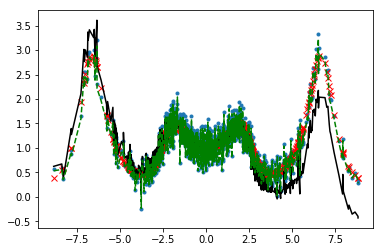
\includegraphics[width=75mm]{4a.png} 
  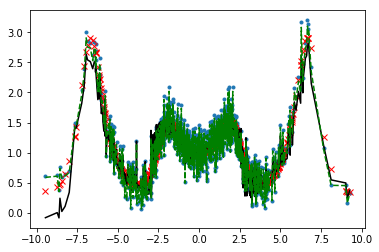
\includegraphics[width=75mm]{4b.png} 


  \textbf{e)} 
  Neurons 20, eta 0.1. Testing set CV score: -1.505540. \\
  This is also a relatively small number of Neurons 
  comparatively. Even though it seems small it looks to
  do a okay job looking at the graph below. The green 
  line seems to represent the data to be able to use to 
  predict it. It is just completely green in the center 
  which means all the data values are accounted for.   \\
  Training set score: 0.935958\\
  Testing set score: 0.933730

  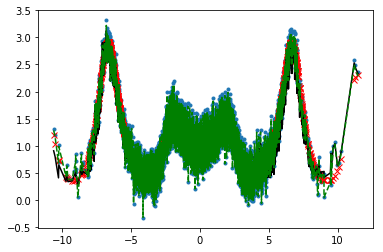
\includegraphics[width=100mm]{4e.png} 
\end{response}


%------------------------------------------------------



\end{document}
%======================================================================================
% END DOCUMENT MAIN BODY ==============================================================
% COPY AND PASTE THIS DOUBLE-SPACE PROBLEM-RESPONSE PAIR AS NEEDED
%======================================================================================



